\subsection{Interações Detalhadas entre Módulos de Grasews}\label{4-grasews-interacoes-detalhadas-modulos}

A \figurename~\ref{fig:grasews-architecture-detailed} detalha as principais interações dos módulos da arquitetura de Grasews. O fluxo da aplicação inicia-se com um usuário interagindo com a interface gráfica da aplicação por meio do módulo  \texttt{Grasews.Web} (à esquerda, na cor azul). \texttt{Grasews.Web} foi desenvolvido utilizando o padrão de arquitetura de desenvolvimento MVC e, portanto, seus principais componentes são representados por \texttt{Models}, \texttt{Views} e \texttt{Controllers}. Um usuário interage com um componente \texttt{View} que, por sua vez, utiliza um objeto modelo definido por um componente \texttt{Model}. A ações de um usuário resultam em eventos controlados por um componente \texttt{Controller}. O componente \texttt{Startup} é responsável por requisitar ao componente \texttt{SimpleInjectorBootstrap} o controle de dependências da aplicação. \texttt{SimpleInjectorBootstrap} (canto inferior, na cor ciano), do módulo \texttt{Grasews.IoC}, é responsável por criar um repositório de referências a objetos (classes) que serão necessários e utilizados por toda a aplicação. Estes objetos tornam-se disponíveis aos demais componentes da aplicação por meio da injeção de dependências realizada nos construtores destes demais componentes. Por fim, um componente de \texttt{Controller} utiliza o componente \texttt{RestClient} para que uma nova requisição seja feita à API da aplicação. O componente \texttt{RestClient} (canto superior, na cor vermelha) é provido pelo módulo \texttt{Grasews.Helpers} (canto superior, na cor cinza claro).

\begin{landscape}
    \begin{figure}[h]
        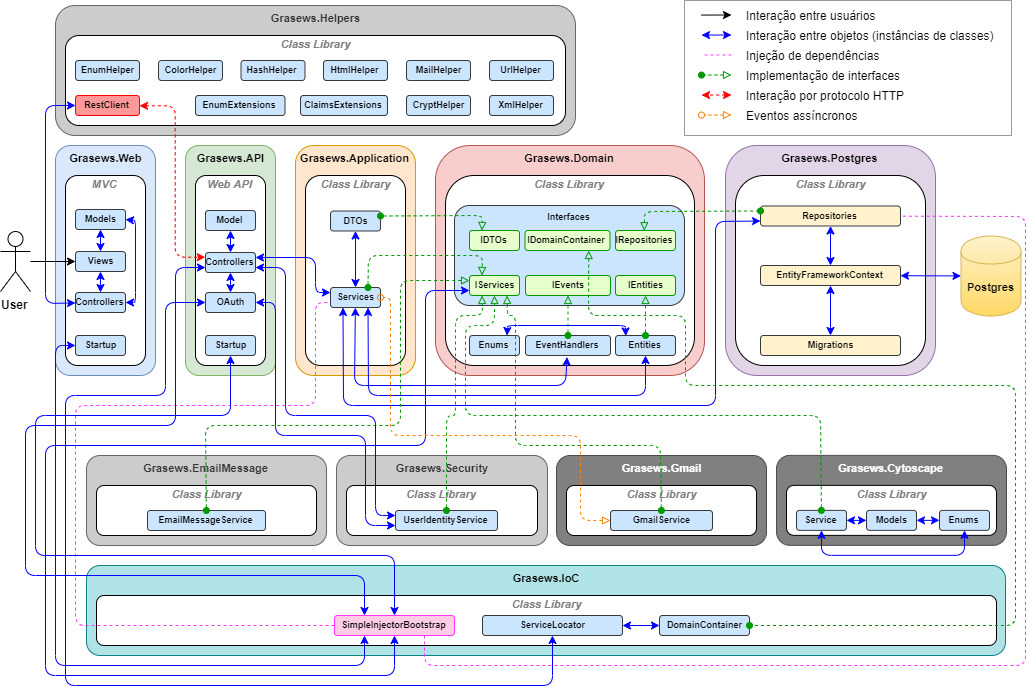
\includegraphics[scale=0.6]{4-grasews/imagens/grasews-architecture-detailed.png}
        \centering
        \caption[Arquitetura do Grasews de forma detalhada]{\textbf{Arquitetura do Grasews de forma detalhada.}}
        \label{fig:grasews-architecture-detailed}
    \end{figure}
\end{landscape}

A API da aplicação é provida pelo módulo \texttt{Grasews.API} (centro à esquerda, na cor verde). Os principais componentes deste módulo são os \texttt{Controllers} e os \texttt{Models}. As requisições originadas de \texttt{Grasews.Web} são gerenciadas por um \texttt{Controller} da API. Tais requisições são repassadas aos serviços do módulo \texttt{Grasews.Application}. Adicionalmente, \texttt{Grasews.API} contém o componente \texttt{Startup}, que assim como no módulo \texttt{Grasews.Web}, este componente é responsável por requisitar o registro de dependências ao módulo \texttt{Grasews.IoC}. Por fim, todos as requisições realizadas para \texttt{Grasews.API} são protegidas. Para realizar uma ação na ferramenta, o usuário deve ser autenticado pelo componente \texttt{OAuth}. Este componente é responsável por validar as credenciais de um usuário, permitindo o uso das funcionalidades da ferramenta, tanto por meio do módulo \texttt{Grasews.Web} quanto do módulo \texttt{Grasews.API}. O componente \texttt{OAuth} utiliza recursos providos por \texttt{UserIdentityService}, do módulo \texttt{Grasews.Security}, localizado no centro inferior do diagrama, na cor cinza claro. Adicionalmente, \texttt{OAuth} utiliza o componente \texttt{ServiceLocator} para obter instâncias de classes que ainda não foram introduzidas no contexto da aplicação pelo componente \texttt{SimpleInjectorBootstrap}. Isso ocorre pelo fato do componente \texttt{OAuth} ser instanciado no início do ciclo da vida da aplicação e não permitir que seu construtor tenha parâmetros de entrada, fator este que possibilita a injeção de dependências. \texttt{ServiceLocator} é auxiliado pelo componente \texttt{DomainContainer}, que atua como um repositório de objetos da aplicação.

O módulo \texttt{Grasews.Application} é representado simplificadamente por meio dos componentes \texttt{Services} e \texttt{DTOs} (\textit{Data Transfer Objects}). As classes que compõem os serviços (\texttt{Services}) são responsáveis por orquestrar todas as requisições originadas do módulo \texttt{Grasews.API}. Requisições realizadas ao módulo \texttt{Grasews.Application} resultam na utilização de objetos das camadas inferiores, como, por exemplo, a criação de instâncias de entidades de domínio, de \texttt{Grasews.Domain}, ou o consumo de métodos de classes de acesso a dados, denominados repositórios, de \texttt{Grasews.Postgres}. Os parâmetros de entrada e de saída de serviços do módulo \texttt{Grasews.Application} variam entre tipos simples, e.g., \textit{int} e \textit{string}, instâncias de entidades de domínio ou então instâncias de um \texttt{DTO}. Nenhum objeto de um tipo de \texttt{Model} de \texttt{Grasews.API} é transferido para \texttt{Grasews.Application}. Os \texttt{Controllers} de \texttt{Grasews.API} são responsáveis por converter seus objetos de tipos de  \texttt{Models} para objetos de tipo de uma entidade de domínio ou então de tipo de um \texttt{DTO}. Desta forma, obtém-se uma melhor segregação do escopo de objetos de cada módulo e, consequentemente, um maior desacoplamento entre os módulos, tornando um módulo o mais autossuficiente possível.

O módulo \texttt{Grasews.Domain} (centro, na cor salmão) contém todas as interfaces (na cor verde claro) de desenvolvimento que são implementadas pelos demais módulos da aplicação. Adicionalmente, \texttt{Grasews.Domain} é responsável por definir as entidades do domínio de negócio da aplicação, representadas pelo componente \texttt{Entities} (na cor azul). Uma entidade geralmente representa uma tabela no banco de dados. Por meio do módulo \texttt{Grasews.Postgres}, estas entidades e suas propriedades são mapeadas para tabelas e colunas do banco de dados, respectivamente. Por fim, \texttt{Grasews.Domain} possui componentes responsáveis por controlar eventos assíncronos. Eventos assíncronos são funcionalidades que podem ser executadas independentemente do fluxo da aplicação, pois não geram dependências para a aplicação. Por exemplo, o envio de um \textit{e-mail} para um usuário pode ser executado de forma assíncrona. Os componentes responsáveis pela implementação do controle de eventos assíncronos são os \texttt{EventHandlers} e as interfaces de \texttt{IEvents}.

O módulo \texttt{Grasews.Postgres} (centro à esquerda, na cor lilás) é responsável por realizar o acesso da aplicação ao banco de dados. Seus principais componentes são os repositórios (\texttt{Repositories}) e o contexto do banco de dados implementado pelo uso do \textit{Microsoft Entity Framework}. O contexto do banco de dados é representado por \texttt{EntityFrameworkContext}. Todas as ações executadas em Grasews que necessitam acesso ao banco de dados são realizadas pelos repositórios. Os repositórios implementam interfaces definidas no módulo \texttt{Grasews.Domain}. Grasews utiliza o SGBD \textit{Postgres} (centro à esquerda, na cor amarelo). Adicionalmente, toda a estrutura de banco de dados de Grasews foi gerada automaticamente por meio do componente \texttt{Migrations} com base nas classes de entidades de domínio existentes no módulo \texttt{Grasews.Domain}. \texttt{Migrations} permite que alterações no modelo do código sejam feitas e depois sejam propagadas no banco de dados.

O módulo \texttt{Grasews.Helpers} (canto superior, na cor cinza claro) possui componentes com funcionalidades que dão suporte a todos os demais módulos de Grasews. Este módulo é composto por diversos componentes com variados propósitos a fim de auxiliar demais objetos da arquitetura da ferramenta. Por fim, o módulo \texttt{Grasews.Cytoscape} (canto inferior direito, na cor cinza escuro) é responsável por manipular nós e arestas do grafo de Grasews. Este módulo foi desenvolvido baseado nas funcionalidades e modelos necessários da biblioteca de desenvolvimento \texttt{Cytoscape.js}, utilizada pelo módulo \texttt{Grasews.Web} para o desenvolvimento dos grafos na interface gráfica de usuário da ferramenta. Os principais componentes de \texttt{Grasews.Cytoscape} são \texttt{Service}, contendo os métodos para manipulação dos elementos (modelos) do grafo, e \texttt{Models}, contendo os tipos de dados necessários para a representação de elementos no grafo, como, por exemplo, nós, arestas e propriedades visuais.